%\documentclass[12pt,a4paper]{beamer}
\documentclass[12pt,a4paper,handout]{beamer}
\usetheme{Amsterdam}
%\usecolortheme{beaver}
\usepackage[english,french]{babel}
%\usepackage[utf8]{inputenc}  
\usepackage[T1]{fontenc}
\usepackage{fontspec}
\usepackage{amsmath}
\usepackage{amsfonts}
\usepackage{amssymb}
\usepackage{tikz}
\usepackage{listings}
\usepackage{pgfplots}
%\pgfplotsset{compat=1.14}
%\pgfplotsset{compat=newest,compat/show suggested version=false}
\pgfplotsset{compat=newest}
\usepackage{color}

%Underline in color
\newcommand{\coloruline}[3]{\emph{\textcolor{#1}{\underline{#2\textcolor{black}{#3}}}}}



\lstset{
  language=Java,
  commentstyle=\color{mygreen},    % comment style
  stringstyle=\color{mymauve},     % string literal style
  keywordstyle=\color{blue},       % keyword style
  basicstyle=\footnotesize        % the size of the fonts that are used for the code
}

\title{\textbf{Algorithmique avancée}}
\subtitle{Introduction aux structures de données}
\author{Frédéric Guyomarch}
\date{2018/2019 - Semestre 3}
\institute % (optional)
{

  IUT-A \\
  Université de Lille

}
 

 
\logo{\includegraphics[width=5em]{figs/iutaustl}}

%Remove Figure prefix on captures
\setbeamertemplate{caption}{\raggedright\insertcaption\par}

%Remove Control bar
\beamertemplatenavigationsymbolsempty

\setbeamertemplate{blocks}[rounded]


\definecolor{mygreen}{rgb}{0,0.6,0}
\definecolor{mygray}{rgb}{0.5,0.5,0.5}
\definecolor{mymauve}{rgb}{0.58,0,0.82}
\definecolor{greenfluo}{rgb}{0,255,0}
\definecolor{blueemph}{RGB}{17,59,94}


\begin{document}

\begin{frame}
\titlepage
\end{frame}

\begin{frame}{Intervenants}
\begin{itemize}
\item Groupe M: Thibault Raffaillac
\item Groupe N: Frédéric Guyomarch
\item Groupe O: Patricia Everaere
\item Groupe L: Thibault Raffaillac
\end{itemize}
\end{frame}


\begin{frame}{Organisation du cours}


\begin{itemize}
\item Volume horaire
\begin{itemize}
\item 16h de TD (2h/semaine)
\item 16h de TP en Java (2h/semaine)... plus vers la fin !
\item 8h de CM (1h/semaine)
\end{itemize}
\item Evaluation
\begin{itemize}
\item un TP noté
\item un examen final
\end{itemize}
\end{itemize}

\end{frame}

%\begin{frame}{Langage Java}
%Utilisation du langage Java dans le cours
%\begin{itemize}
%\item Langage orienté objet
%\item Pas de pointeurs
%\item Ramasse-miettes
%\end{itemize}
%\end{frame}
\begin{frame}{Des structures...}
{de données!}

Les données sont \textit{partout}, parfois \textit{complexes} et souvent \textit{structurées} par nature!
        \pause

 \begin{figure}
        \centering
        \begin{minipage}{.50\textwidth}
            \centering
            \includegraphics[width=0.9\linewidth]{figs/dico.jpg}
          \caption{Dictionnaire}
        \end{minipage}%
        \pause
        \begin{minipage}{.50\textwidth}
            \centering
            \includegraphics[width=0.8\linewidth]{figs/map.png}
            \caption{Une carte}
        \end{minipage}
  
    \end{figure}



\end{frame}



\begin{frame}{Introduction aux structures de données}
{}
\begin{definition}
Une structure de données (SDD) est un agencement, une manière d'organiser les données en mémoire.
\end{definition}

\pause
\vspace{25pt}
\emph{Algorithms + Data Structures = Programs (Niklaus Wirth)}

\end{frame}


\begin{frame}{Introduction aux structures de données}
{Objectifs de la matière}
\begin{itemize}
\item Découvrir les principales structures de données (SDD),
\item ainsi que les algorithmes associés, 
\item savoir les modéliser,
\item pour au final utiliser les SDD adaptées aux problèmes.
\end{itemize}

\end{frame}



%\begin{frame}{Les types de données abstraits}
%
%\begin{definition}
%Un type de données abstrait (TDA) est une spécification de données et des opérations réalisables sur ces données.
%\end{definition}

%\begin{itemize} 
%\item La spécification est \textbf{indépendante} de l'implémentation
%\item Analogie avec les classes du paradigme objet
%\end{itemize}
%
%\end{frame}
%
%\begin{frame}{Les types de données abstraits}
%{Exemple de la voiture}
%
%\begin{figure}
%\includegraphics[scale=2]{figs/car} 
%\end{figure}
%
%
%\end{frame}
%
%\begin{frame}{Les types de données abstraits}
%{Exemple de la voiture}
%
%\begin{figure}
%\includegraphics[scale=0.4]{figs/car1} 
%\end{figure}
%
%
%\end{frame}
%
%\begin{frame}{Les types de données abstraits}
%{Exemple de la voiture}
%
%\begin{figure}
%\includegraphics[scale=0.4]{figs/car2} 
%\end{figure}
%\vspace{-2em}
%L'interface correspond aux opérations possibles sur le TDA voiture.
%
%\end{frame}


%\begin{frame}{Introduction aux structures de données}{}
%
%
%Opérations courantes sur les structures de données:
%\begin{itemize}
%\item Rechercher un élément
%\item Ajouter un élément
%\item Supprimer un élément
%\end{itemize}
%


%\end{frame}


\begin{frame}{Introduction aux structures de données}{Contenu de la matière}
\begin{itemize}
\item Algorithmes de tris
\item Listes chaînées
\item Piles/Files
\item Tables de hachage
\item Arbres binaires
\end{itemize}
\end{frame}


\begin{frame}{Introduction aux structures de données}{Une classification grossière des SDD}
\begin{itemize}
\item Stockage de données réelles (listes chaînées, tables de hachage, etc)
\item Outils de programmeurs pour les programmeurs (files avec priorités, piles, etc.)
\item Modélisation (graphes, files,etc.)
\end{itemize}
\end{frame}



\begin{frame}[fragile]{Rappel sur les tableaux}{En Java}

\begin{lstlisting}
/*Declaration d'un tableau d'entiers */
int [] tab;
/*Allocation de ce tableau de taille 10 */
tab = new int[10];
\end{lstlisting}

\begin{figure}
\centering
\includegraphics[scale=0.3]{figs/array_empty}
\end{figure}

\end{frame}

%% à revoir
\begin{frame}{Rappel sur les tableaux}{Insertion}

Ajouts successifs des valeurs 22, 11, 8, 17, 25, 34, 47, 52, 69 et 98.

\only<1>{
\begin{figure}
\centering
\includegraphics[scale=0.3]{figs/array_empty}
\end{figure}
} 

\only<2>{
\begin{figure}
\centering
\includegraphics[scale=0.3]{figs/array_0}
\end{figure}
} 

\only<3>{
\begin{figure}
\centering
\includegraphics[scale=0.3]{figs/array_1}
\end{figure}
} 

\only<4>{
\begin{figure}
\centering
\includegraphics[scale=0.3]{figs/array_2}
\end{figure}
} 

\only<5>{
\begin{figure}
\centering
\includegraphics[scale=0.3]{figs/array_3}
\end{figure}
} 

%\only<6>{
%\begin{figure}
%\centering
%\includegraphics[scale=0.3]{figs/array_4}
%\end{figure}
%} 

%\only<7>{
%\begin{figure}
%\centering
%\includegraphics[scale=0.3]{figs/array}
%\end{figure}
%} 

%\pause
\vspace{-0.4cm}
Il suffit d'incrémenter un compteur pour placer chaque valeur au bon endroit.

\end{frame}
\begin{frame}[fragile]{Rappel sur les tableaux}{Recherche Séquentielle}

Recherche de la valeur 47:


\begin{figure}
\centering
\includegraphics[scale=0.3]{figs/array}
\end{figure}

\pause
\begin{lstlisting}[tabsize=2,showtabs]
int search(int val, int[] tab){
  for(int i=0; i < tab.length; ++i){
    if(tab[i]==val){
     return i;
    }
  }
 return -1;
}

\end{lstlisting}
\pause
 \begin{center}
   \textcolor{blueemph}{\textbf{Dans le pire cas $n$ itérations...
}}
   \end{center} 

\end{frame}

\begin{frame}[fragile]{Rappel sur les tableaux}{Recherche Séquentielle}
\begin{figure}
\centering
\includegraphics[scale=0.3]{figs/array}
\end{figure}

\pause
\begin{lstlisting}[tabsize=2,showtabs]
int search(int val, int[] tab){
  for(int i=0; i < tab.length && tab[i] != val ; ++i);
  if (i==tab.length)
    return-1;
  else
    return i;
}

\end{lstlisting}
\pause
 \begin{center}
   \textcolor{blueemph}{\textbf{Version plus élégante !}}
  \end{center} 

\end{frame}

%% à revoir
\begin{frame}{Rappel sur les tableaux}{Suppression}

Suppression (sans trou dans le tableau) de la valeur 47:

\only<1>{
\begin{figure}
\centering
\includegraphics[scale=0.3]{figs/array_search_47}
\end{figure}
} 


\only<2>{
\begin{figure}
\centering
\includegraphics[scale=0.3]{figs/array_delete_47A}
\end{figure}
} 

\only<3>{
\begin{figure}
\centering
\includegraphics[scale=0.3]{figs/array_delete_47B}
\end{figure}
} 

\only<4>{
\begin{figure}
\centering
\includegraphics[scale=0.3]{figs/array_delete_47C}
\end{figure}
} 

\only<5>{
\begin{figure}
\centering
\includegraphics[scale=0.3]{figs/array_delete_47D}
\end{figure}
} 


\only<6>{
\begin{figure}
\centering
\includegraphics[scale=0.3]{figs/array_delete_47E}
\end{figure}
} 

\begin{itemize}

\onslide<2-6>{\item[1] Recherche de la valeur 47 (index $i=6$)}
\onslide<3-6>{\item[2] Décalage de -1 pour les cases d'index $i+1$ à $n-1$}

\end{itemize}


\end{frame}




\begin{frame}{Tableau ordonné}{Insertion}

Ajouts successifs des valeurs 22, 11, 8, 17, 25, 34, 47, 52, 69 et 98.

\only<1>{
\begin{figure}
\centering
\includegraphics[scale=0.3]{figs/array_empty}
\end{figure}
} 

\only<2>{
\begin{figure}
\centering
\includegraphics[scale=0.3]{figs/array_0}
\end{figure}
} 

\only<3>{
\begin{figure}
\centering
\includegraphics[scale=0.3]{figs/array_ord_1}
\end{figure}
} 
\only<4>{
\begin{figure}
\centering
\includegraphics[scale=0.3]{figs/array_ord_2}
\end{figure}
} 

\only<5>{
\begin{figure}
\centering
\includegraphics[scale=0.3]{figs/array_ord_3}
\end{figure}
} 
\only<6>{
\begin{figure}
\centering
\includegraphics[scale=0.3]{figs/array_ord_4}
\end{figure}
} 

\only<7>{
\begin{figure}
\centering
\includegraphics[scale=0.3]{figs/array_ord}
\end{figure}
} 



Chaque valeur doit être re-positionnée à la bonne place à chaque insertion

\end{frame}

\begin{frame}{Tableau ordonné}{Recherche}
\begin{itemize}
\item Recherche séquentielle inefficace
\item Utilisation du caractère trié du tableau
\item Principe de la \textcolor{blueemph}{\textbf{recherche dichotomique}}
\end{itemize}

\end{frame}

\begin{frame}{Tableau ordonné}{Recherche dichotomique}

\only<1>{
Recherche de la valeur 47:

\begin{figure}
\centering
\includegraphics[scale=0.3]{figs/array_dicho}
\end{figure}
} 

\only<2>{
\begin{figure}
\centering
\includegraphics[scale=0.3]{figs/array_dicho1}
\end{figure}
} 


\only<3>{
\begin{figure}
\centering
\includegraphics[scale=0.3]{figs/array_dicho15}
\end{figure}
} 


\only<4>{
\begin{figure}
\centering
\includegraphics[scale=0.3]{figs/array_dicho2}
\end{figure}
} 

\only<5>{
\begin{figure}
\centering
\includegraphics[scale=0.3]{figs/array_dicho25}
\end{figure}
} 

\only<6>{
\begin{figure}
\centering
\includegraphics[scale=0.3]{figs/array_dicho3}
\end{figure}
} 

\only<7>{
\begin{figure}
\centering
\includegraphics[scale=0.3]{figs/array_dicho35}
\end{figure}
} 


\only<8>{
\begin{figure}
\centering
\includegraphics[scale=0.3]{figs/array_dicho4}
\end{figure}
} 

\only<2>{
 \begin{minipage}[c]{.55\linewidth}
  \begin{itemize}
\item début = 0
\item fin = 9
\item milieu = (début+fin/2) = 4
\end{itemize}
   \end{minipage} \hfill
   \begin{minipage}[c]{.35\linewidth}
     tab[milieu] < 47
   \end{minipage} 
}
\only<3>{
 \begin{minipage}[c]{.55\linewidth}
  \begin{itemize}
\item début = 0
\item fin = 9
\item milieu = (début+fin/2) = 4
\end{itemize}
   \end{minipage} \hfill
   \begin{minipage}[c]{.35\linewidth}
     tab[milieu] < 47 \newline $\Rightarrow$ 47 est en \colorbox{greenfluo}{partie droite}
   \end{minipage} 
}

\only<4>{
 \begin{minipage}[c]{.55\linewidth}
  \begin{itemize}
\item début = milieu + 1 = 5
\item fin = 9
\item milieu = (début+fin/2) = 7
\end{itemize}
   \end{minipage} \hfill
   \begin{minipage}[c]{.35\linewidth}
     tab[milieu] > 47 
   \end{minipage} 
}


\only<5>{
 \begin{minipage}[c]{.55\linewidth}
  \begin{itemize}
\item début = milieu + 1 = 5
\item fin = 9
\item milieu = (début+fin/2) = 7
\end{itemize}
   \end{minipage} \hfill
   \begin{minipage}[c]{.35\linewidth}
     tab[milieu] > 47 \newline $\Rightarrow$ 47 est en \colorbox{greenfluo}{partie gauche}
   \end{minipage} 
}




\only<6>{
 \begin{minipage}[c]{.55\linewidth}
  \begin{itemize}
\item début = 5
\item fin = milieu - 1 = 6
\item milieu = (début+fin/2) = 5
\end{itemize}
   \end{minipage} \hfill
   \begin{minipage}[c]{.35\linewidth}
     tab[milieu] < 47 
   \end{minipage} 
}

\only<7>{
 \begin{minipage}[c]{.55\linewidth}
  \begin{itemize}
\item début = 5
\item fin = milieu - 1 = 6
\item milieu = (début+fin/2) = 5
\end{itemize}
   \end{minipage} \hfill
   \begin{minipage}[c]{.35\linewidth}
     tab[milieu] < 47 \newline $\Rightarrow$ 47 est en \colorbox{greenfluo}{partie droite}
   \end{minipage} 
}


\only<8>{
 \begin{minipage}[c]{.55\linewidth}
  \begin{itemize}
\item début = milieu + 1 = 6
\item fin = 6
\item milieu = (début+fin/2) = 6
\end{itemize}
   \end{minipage} \hfill
   \begin{minipage}[c]{.35\linewidth}
     tab[milieu] = 47 \newline $\Rightarrow$ 47 est trouvé
   \end{minipage} 
 
 
 \pause
   \vspace{1em}
   \begin{center}
   \textcolor{blueemph}{\textbf{Au pire $log_2 n$ itérations}}
   \end{center}  
   
}



\end{frame}

%\begin{frame}{Comparaison}{}
%
% \begin{minipage}[c]{.45\linewidth}
%Tableau
%\begin{itemize}
%\item Insertion rapide
%\item Recherche lente
%\end{itemize}
%   \end{minipage} \hfill
%   \begin{minipage}[c]{.45\linewidth}
%   Tableau ordonné
%   \begin{itemize}
%\item Insertion lente
%\end{itemize}
%   \end{minipage} 
%
%\end{frame}




\begin{frame}{Comparaison}
\begin{itemize}
\item L'insertion est plus rapide dans le tableau non ordonné.
\item La recherche est beaucoup plus rapide dans un tableau ordonné.
\item La suppression d'une valeur (recherche inclue) prend un temps équivalent dans les deux cas (sinon plus rapide).
\end{itemize}
\pause
Quelle est la meilleure des deux SDD?\newline
\pause
\begin{center}
\textcolor{blueemph}{\textbf{Ça dépend de la situation!}}
\end{center}
\end{frame}

\begin{frame}{Tableau ordonné ou non ordonné?}
Un tableau ordonné serait plus adapté pour un registre d'employés:
\begin{itemize}
\item car peu d'ajouts,
\item mais des recherches fréquentes.
\end{itemize}
Et un tableau non ordonné à un historique des achats:
\begin{itemize}
\item car insertions fréquentes,
\item mais recherches plus rares.
\end{itemize}

\end{frame}




\begin{frame}{Les types de données abstraits}

\begin{definition}
Un type de données abstrait (TDA) est une spécification de données et des opérations réalisables sur ces données.
\end{definition}

\begin{itemize} 
\item La spécification est \textbf{indépendante} de l'implémentation
\item Analogie avec les classes du paradigme objet
\end{itemize}

\end{frame}

\begin{frame}{Les types de données abstraits}
{Exemple de la voiture}

\begin{figure}
\includegraphics[scale=2]{figs/car} 
\end{figure}
\end{frame}

\begin{frame}{Les types de données abstraits}
{Exemple de la voiture}

\begin{figure}
\includegraphics[scale=0.4]{figs/car1} 
\end{figure}


\end{frame}

\begin{frame}{Les types de données abstraits}
{Exemple de la voiture}

\begin{figure}
\includegraphics[scale=0.4]{figs/car2} 
\end{figure}
\vspace{-2em}
L'interface correspond aux opérations possibles sur le TDA voiture.
\end{frame}


\begin{frame}{TDA Tableau}
\begin{figure}
\centering
\includegraphics[scale=0.4]{figs/ADTtableau} 
\end{figure}
\end{frame}

\begin{frame}{Opérations}
Généralement on retrouvera dans les TDA:
\begin{itemize}
\item une opération d'insertion,
\item une opération de recherche,
\item une opération de suppression.
\end{itemize}

\end{frame}

\begin{frame}{Java Framework Collections}
Ensemble de classes et interfaces (les TDA) pour les structures de données en Java.

\begin{figure}
\centering
\includegraphics[scale=0.4]{figs/framework_collections_java} 
\end{figure}



\end{frame}

\begin{frame}{(R)appel}{La généricité}

\begin{itemize}
\item Élimine plus d'erreurs à la compilation par vérification de type
\item Permet de se passer de transtypage (cast)
\item Agit par paramétrage de type
\item Permet d'écrire des algorithmes fonctionnant avec tous les types
\pause \item[$\Rightarrow$] + d'abstraction
\end{itemize}




\end{frame}

\begin{frame}[fragile]

Sans généricité
\begin{lstlisting}
List list = new ArrayList();
list.add("hello N3");
String s = (String) list.get(0);
\end{lstlisting}
\pause

Avec:
\begin{lstlisting}
List<String> list = new ArrayList<String>();
list.add("hello N3");
String s = list.get(0);   // pas de transtypage
\end{lstlisting}

\end{frame}


\begin{frame}[fragile]
Une classe non générique:
\begin{lstlisting}
public class Box {
    private Object object;

    public void set(Object object) { 
      this.object = object; 
    }
    public Object get() { return object; }
}
\end{lstlisting}

\end{frame}

\begin{frame}[fragile]
Une classe générique paramétrée:
\begin{lstlisting}
public class Box<T> {
    private T t;   // T pour "Type" par convention

    public void set(T t) {
     this.t = t; 
    }
    public T get() { return t; }
}
\end{lstlisting}
\pause
Invocation:
\begin{lstlisting}
Box<Integer> integerBox = new Box<Integer>();
\end{lstlisting}

\end{frame}

\begin{frame}{Bilan}
Nous avons vu dans ce cours:
\begin{itemize}
\item Le fonctionnement de la matière pour le semestre,
\item pourquoi utiliser des SDD,
\item qu'il faut choisir une structure adaptée à sa situation,
\item et la notion de type de données abstrait.
\end{itemize}
\end{frame}

\end{document}